\section{Experiment Evaluation}
\label{sec:experiment}
In this section, we first give some statistics of our dataset and evaluate the quality and quantity of the learned rules. Then, we compare ours with other causal knowledge bases. Next, we analyze and discuss some main sub-modules in the rule learning framework. Finally, a practical application of [futures price prediction] and demonstration are introduced. Our experiments are implemented in Python and SWI-Prolog.
% and run on a computer with Intel Xeon 32 CPU(2.60GHz) and 173GB memory.
	
\subsection{Dataset}
We crawled the text dataset from Chinese financial news website.\footnote{\url{ http://finance.sina.com.cn}} The news data containing 4,991,000 articles, from 2000/7/20 to 2017/12/31, is used to rule learning.
%	, which are split into \textbf{111,330,205} sentences. The number of unique sentences is \textbf{75,572,053}, covering  \textbf{67.88\%} of the total sentences. 
The number of sentences with causal cue words is 7,147,141, accounting for 9.46\% of the total number of de-duplicated sentences (75,572,053. The repetition rate of sentences is about 32\%).
It shows that about  \textbf{14.2\%} (9.64\%/(1-32\%)) sentences explicitly express causality in online financial news sentences.
%The news data containing 270,562 articles, from 2018/1/1 to 2018/11/2, is used to evaluate our framework. 
We set $\alpha$ to 0.5 to achieve an equal balance between generalization and specialization in rule induction. 
After a lot of experimental reasoning observations, we set $\gamma$ to 0.3 to control the Prolog engine to reason around two steps.

%	\begin{table}[]
%		\caption{Dataset Information}
%		\begin{center}
%		\begin{tabular}{|l|l|l|}
%			\hline
%			Dataset       & Train & Test \\ \hline
%			Time Interval &       &      \\ \hline
%			Number        &       &      \\ \hline
%		\end{tabular}
%	\end{center}
%	\end{table}

\subsection{Rule Evaluation}
In this section, we evaluate these rules both quantitatively and qualitatively.
\paragraph{Quantitative Evaluation}
The number of the final rules we learned is \textbf{42,037}. We divide the rule quality into three levels: good, fair and bad. According to the ranking of rule confidence, we randomly select 200 rules from the top 10000 rules and manually divide them into three levels: good, fair and bad. The 'good' means the rules are causally correct, 'bad' means the rules are causally incorrect (e.g., an event should cause the price of something to rise, but the rule indicates that its price falls.) and 'fair' means that the causality in the general rule is vague and hard to tell. In the first 10,000 rules, a total of 42,037 rules have been learned, good: 50.5\%, Fair: 39.5\%, bad: 10\%, respectively.
\begin{figure}[htbp]
	\centering
	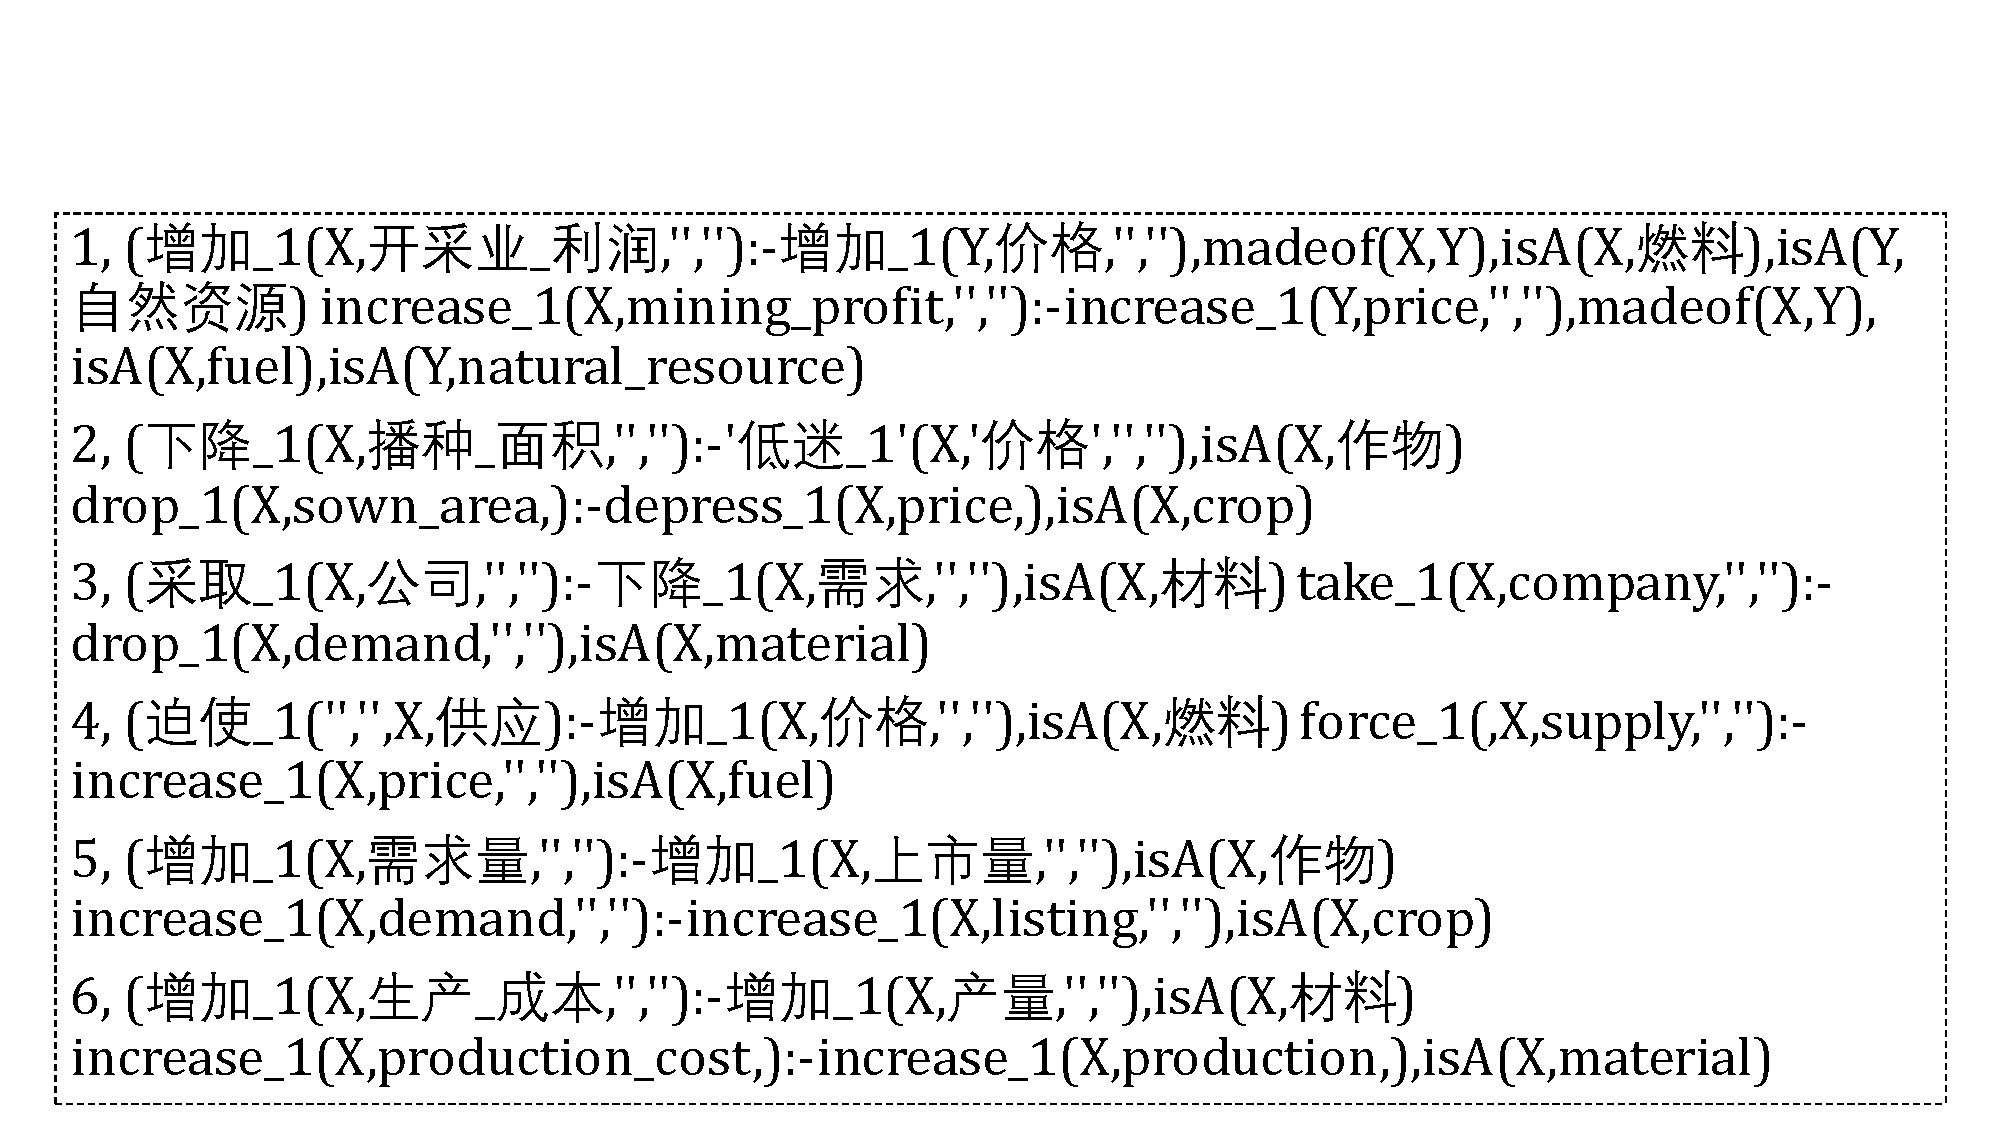
\includegraphics[width=0.95\columnwidth]{figures/rules_case}
	\caption{Examples of Typical Rules}
	\label{fig:rules_case}
\end{figure}
\paragraph{Qualitative Evaluation}
%\begin{align*}
%%	good
%%	{"c": ["过剩_1", "X_燃料", "产量", "", ""], "e": ["下降_1", "X_自然资源", "价格", "", ""], "relation": [["c_sc", "e_sc", "madeof"]], "ctx": {"senids": [1975666], "pattern_ids": [8]}, "ruleid": 5131, "confidence": 0.5657637042081998}
%&\text{1 (X, '产量/yield', '过剩/surplus', '', ''):-(Y, '价格/price', '下降/fall',} \nonumber\\
%&\text{'',''), IsA(X, '燃料/fuel'), IsA(Y, '自然资源/natural resource'),} \nonumber\\
%&\text{madeof(X, Y)} \\
%%{"c": ["结束_1", "X_国家", "罢工", "", ""], "e": ["下降_1", "X_金属", "价格", "", ""], "relation": [["e_sc", "c_sc", "atlocation"]], "ctx": {"senids": [341012], "pattern_ids": [6]}, "ruleid": 11607, "confidence": 0.5824045924950126}
%&\text{2 (X, '罢工/strike', '结束/stop', '', ''):-(Y, '价格/price', '下降/fall', }\nonumber\\
%&\text{'',''), IsA(X, '国家/nation'), IsA(Y, '金属/metal')}\nonumber\\
%&\text{, atlocation(Y, X)}	 \\
%%{"c": ["下降_1", "X_作物", "价格", "", ""], "e": ["减少_1", "", "", "X_作物", "面积"], "relation": [["c_sc", "e_oc", "=="]], "ctx": {"senids": [961411], "pattern_ids": [8]}, "ruleid": 978, "confidence": 0.5876590112986869}
%&\text{3 (X, '价格/price', '下降/fall', '', ''):-(X, '面积/area', '减少/fall', }\nonumber\\
%&\text{'',''), IsA(X, '作物/crop')} \\
%%fair
%%2{"c": ["下降_1", "X_国家", "储蓄率", "", ""], "e": ["下降_1", "X_国家", "增长率", "", ""], "relation": [["c_sc", "e_sc", "=="]], "ctx": {"senids": [1640122], "pattern_ids": [5]}, "ruleid": 213, "confidence": 0.7185889172176277}
%&\text{4 (X, '储蓄率/saving rate', '下降/fall', '', ''):-(X, '增长率/growth rate', }\nonumber\\
%&\text{'下降/fall','',''), IsA(X, '国家/nation')} \\
%%2{"c": ["下降_1", "", "X_产品", "", ""], "e": ["适合_1", "", "X_作物", "", ""], "relation": [["c_s", "e_s", "madeof"]], "ctx": {"senids": [1791763], "pattern_ids": [6]}, "ruleid": 19783, "confidence": 0.5634539402859007}
%&\text{5 ('', X, '下降/fall', '', ''):-('', Y, '适合/fit', '', ''), IsA(X, }\nonumber\\
%&\text{'产品/product'), IsA(Y, '作物/crop'), madeof(X, Y)}   \\
%%bad
%%1{"c": ["减少_1", "", "X_国家", "X_自然资源", "依赖性"], "e": ["增加_1", "", "", "X_燃料", "销量"], "relation": [["e_oc", "c_oc", "madeof"]], "ctx": {"senids": [1707156], "pattern_ids": [8]}, "ruleid": 4468, "confidence": 0.5717182258485046}
%%另一方面,由于日本、韩国和中国减少对中东地区进口原油的依赖性,道达尔公司希望增加对这三个国家的液化天然气销量。
%&\text{6 ('', X, '减少/fall', Y, '依赖性/dependence'):-('', '', '增加/increase',}\nonumber\\
%&\text{ Z,'销量/sales'), IsA(X, '国家/nation'), IsA(Y, '自然资源/natural-} \nonumber\\
%&\text{resource'), IsA(Z, '燃料/fuel'), madeof(Z,Y)}	
%\end{align*}
Figure \ref{fig:rules_case} shows some typical rules: 1,2 are good, 3,4 are fair, and 5,6 are bad.
The main problems of these rules include:
The extracted events are incomplete, which makes the rules less informative, such as rule 3,4.
and the logics of causation in both rule 5 and rule 6 are wrong.

Some other problems also exist, such as insignificant causality caused by the loose causal patterns, verb disambiguation when normalizing predicates, noun disambiguation when generalizing rule instances.

\begin{table*}[htbp]
\centering
	\begin{tabular}{|c|c|c|c|c|c|c|c|}\hline
	\textbf{Name}&\textbf{Number}&\textbf{Domain}&\textbf{Data/Structured}&\textbf{Exp}&\textbf{Source}&\textbf{Unc}&\textbf{Accuracy}\\ \hline
	CausalNet&\textbf{62,675,002}&\textbf{Open}&word/\textbf{Yes}&bad&\textbf{automatic}&No&-\\
	\multicolumn{8}{|c|}{(`drink',`accident',36)}\\\hline
	ConceptNet &89,416&\textbf{Open}&short text/No&fair&crowdsource&No&\textbf{100\%}\\
	\multicolumn{8}{|c|}{(`smoking',`/r/Causes',`cancer')}\\\hline
	FrameNet&59&\textbf{Open}&frame/\textbf{Yes}&fair&crowdsource&No&\textbf{100\%}\\
	\multicolumn{8}{|c|}{Killing(Killer,Place,Means,Victim,Instrument),CausativeOf,Death(Protagonist,Place,Manner,Time)}\\\hline
	BECauSE 2.0 &1803&\textbf{Open}&text/No&good&crowdsource&No&\textbf{100\%}\\
	\multicolumn{8}{|c|}{(we don’t have much time, so let’s move quickly.)}\\\hline
	ATOMIC&568,312&\textbf{Open}&\textbf{logic event}/No&good&crowdsource&No&86.2\%\\
	\multicolumn{8}{|c|}{If ``PersonX pays PersonY a compliment", Then ``PersonY will smile"}\\\hline
	Ours&42,037&Finance&\textbf{logic event}/\textbf{Yes}&\textbf{best}&\textbf{automatic}&\textbf{Yes}&50.5\%\tablefootnote{This is the accuracy of top 10000 rules.}\\ 
%			Deductive Rule Instance&\TD{??}\\ 
%	\multicolumn{8}{|c|}{See above rule example in Figure\ref{fig:rules_case}}\\\hline

	\multicolumn{8}{|c|}{
			\begin{tabular}{c}
		rise(Z,price,`',`'):-suffer(`',X,Y,attack),isA(X,country),isA(Y,disaster),isA(Z,metal),\\atLocation(Z,X) conf:0.842\end{tabular}}\\\hline

%	\multicolumn{8}{|c|}{
%		\begin{tabular}{c}
%			rise(Z,price,`',`'):-suffer(`',X,Y,attack),isA(X,country),isA(Y,disaster),isA(Z,metal),\\
%			atLocation(Z,X) conf:0.842
%		\end{tabular}}\\\hline	
		\end{tabular}

\caption{Comparison with existing knowledge bases(Exp means Expressiveness, Unc means Uncertainty)}
\label{tab:comparison_rule_with_kbs}
\end{table*}


\subsection{Comparison with existing resources}
We compare our rules with causal relation of other knowledge bases in various aspects in Table \ref{tab:comparison_rule_with_kbs}. It shows our causal knowledge representation is more expressive, because each rule can express a kind of causal event. Besides, the automatic knowledge acquisition is effective, and probabilistic features are used to express knowledge uncertainty. What's more, our rule learning is easy to extend to the open domain.


%\begin{table}[htbp]
%	\caption{Rule Instance \& Rule}
%	\begin{center}
%	\begin{tabular}{|r|l|}\hline
%		\multicolumn{1}{|c|}{Name}                  & \multicolumn{1}{c|}{Number} \\\hline
%		\multicolumn{1}{|c|}{Rule Instances}        & \multicolumn{1}{c|}{7835403} \\ \hline
%		\multicolumn{1}{|c|}{Rules}                 & \multicolumn{1}{c|}{69036}  \\ \hline
%		\multicolumn{1}{|c|}{more than on relation} & \multicolumn{1}{c|}{2499(3.6\%)}\\
%		\multicolumn{1}{|c|}{only one relation}     & \multicolumn{1}{c|}{66539(96.4\%)} \\
%		\hline
%		==                                          & 56449(84.8\%)                      \\
%		madeof                                      & 5659(8.5\%)                        \\
%		atlocation                                  & 1835(2.76\%)                       \\
%		partof                                      & 1061(1.59\%)                       \\
%		usedfor                                     & 954(1.43\%)                        \\
%		hasa                                        & 511(0.768\%)                       \\
%		derivedfrom                                 & 38(0.0571\%)                       \\
%		hasproperty                                 & 20(0.0301\%)                       \\
%		createdby                                   & 12(0.018\%)                        \\ \hline
%	\end{tabular}
%	\label{tab:rule_statistics}
%\end{center}
%\end{table}
	%Rule Instances & 1817014(4337755)\\
	%Candidate Rules & 86218(201359)\\
	%Rule & 18348(42246)\\
\subsection{Ablation Study}
In this section, we explore the contributions of various components of our rule learning framework.
\paragraph{Causal patterns statistic} The matched sentences distribution over 3 groups of patterns is shown in Table \ref{tab:pattern_statistics}. All patterns in one group have different causal cue words literally but the same meaning. It shows the third pattern group is more rigorous than the first two groups but has lower usage. This is probably because that more logical thinking is needed, if using more rigorous patterns, when editing news.

\begin{table}[htbp]
	\centering
	\begin{tabular}{|c|c|c|c|} \hline
		\textbf{Pattern template}& \textbf{Pri}&\textbf{Number}& \textbf{Rate}\\	\hline 
		因为 A,B&1&2000242&48.32\% \\ \hline 
		A,所以 B&2&1530311&36.96\% \\ \hline 
		因为 A, 所以B&3&576851&14.72\% \\	\hline
	\end{tabular}
	\caption{Number of sentences extracted by causal patterns. A is a cause span and B is an effect span. Word `因为' represents a group works like 由于,是因为,因为,缘于,归因于,原因是,鉴于, and word `所以' represents a group of words like 所以,因而,因此,故而,因故,导致,招致,以致,引致,诱致,致使,造成,使得,从而使,于是,为此. (Pri means Priority)}
	\label{tab:pattern_statistics}
\end{table}	
\paragraph{External Knowledge Bases}
The following is some statistics of external knowledge bases used in the rule learning framework. The size of the lexicon is 12,624, obtained from `Industrial classification for national economic activities'\footnote{\url{ http://www.stats.gov.cn/Tjsj/tjbz/hyflbz/}}, which determines which event role in the rule instance can be generalized. 
We use the Google translator\footnote{\url{https://translate.google.com}} to translate both English Probase and English ConceptNet. We concatenate the two terms from the triple into one phrase and throw this phrase to Google translator , and then split the translated result string into two separate Chinese terms to get \zhpro and \zhcon.
\zhpro has 11,292,493 Chinese `IsA' pairs and
\zhcon 2,085,681 Chinese triples.
We randomly sample 500 items from translated Probase and ConceptNet, respectively, and the accuracies after the human evaluation are \textbf{87.8\%} (close to the accuracy of original Probase 92.6\%) and \textbf{91.6\%}.

%\begin{table}[htbp]
%	\centering
%	\begin{tabular}{|c|c|}\hline
%		\textbf{Name}&\textbf{Number}\\ \hline
%		Lexicon&12624\\ \hline
%		Translated Probase &11,292,493(87.8\%)\\ \hline
%		Translated ConceptNet&2,085,681(91.6\%)\\ \hline
%	\end{tabular}
%	\caption{External Knowledge Bases}
%	\label{tab:knowledge_base_statistics}
%\end{table}

%After translation, the number of Chinese IsA pairs is 11,292,493. The number of Chinese commonsense triples is 2,085,681. We both randomly sample 500 items from them, and the accuracy after human evaluation are 0.878 and 0.916 respectively.
%The accuracy of original Probase is 0.926. 
%The number of total Chinese IsA pairs are 11,292,493 which contain concept-instance pairs and concept-subconcept pairs, the. The number of Chinese concepts is 81082 concluding concepts and subconcepts. The number of instances is 158693. The number of Chinese commonsense pairs is 7316977.
%\subsection{External Factual Knowledge Bases}

%From above rule instance extraction submodule, we scan get a rule instances repository. With such huge specific rule instances, we hope to further discover the powerful knowledge hidden in these rule instances. 

%so we generalize such a large amount of rule instances with a more general form. As discussed in Section \ref{sec:intro}, we need to build such a knowledge base. Taxonomy and common sense are two major kinds of knowledge in such knowledge base.
%In our framework, we need to rely on the external Chinese knowledge bases, Chinese Probase and Chinese Conceptnet, to generalize rule instances and add constraints. Most existing Chinese taxonomy knowledge is constructed from online-encyclopedia, such as CN-Probase\cite{Xu2017}. They usually focus more on named entity such as famous movie stars, singer stars, while we care more about the concrete things existed in life such as corn, steel, alcohol and so on.  In addition, they have no probabilistic character. Translation is an effective and efficient approach, we choose to translate Probase, which is a probabilistic taxonomic knowledge base.
%To our knowledge, there exists no large-scale Chinese commonsense knowledge base, so we translate the English part of ConceptNet5 into Chinese and combine the Chinese part.

%	 which is special for this, But it is only for English. We have investigated the CN-Probase\cite{xu2017cn}, but It even can't find the concept of common entities like '中国/China', '橡胶/rubber' and it also limits the usage frequency. So we collect the items from Probase, the items with 'IsA' relation in ConceptNet5\cite{speer2013conceptnet}, Webbrain\cite{chen2016webbrain}. Then, we fuse them together, Then, translate them into Chinese with google translator. to reduce the translate error, we put more context into the translator as more as possible, for example we put 'fruit such as apple, banana', Then we can get the translated result of IsA(apple,fruit), IsA(banana, fruit) together, which can make word sense of 'apple' to be translated near the fruit not company.  
%	\subsubsection{Chinese Commonsense knowledge base.}
%	, consisting of 47, 3, 25 relations respectively. Some of them are duplicative and some are useless for us. So we select specific number useful relations and we also design some patterns to extract some relations from Chinese wiki. 
%	relattions between arguments are used in rule specialization submodule to make rules reasonable. There exist many commonsense knowledge bases such as ConceptNet5, WebBrain, WebChild.  The numbers of the relations in these knowledge bases are limited. And some relations are equivalent among different knowledge bases, such as '/r/RelateTo' in ConceptNet is equivalent to 'relateto' in WebBrain. So we normalize all the relations names literally.
% Meanwhile, many pairs of arguments have more than one relations which are  duplicated semantically. For example, (sweet corn, corn) has the relations 'relatedto' and 'partof', obviously, 'partof' consists of 'relatedto' semantically. So we hope to remove the semantic reduplication relations. which means we need find the semantic containment relations among these relations.
%Algorithm \ref{alg:alg1} shows the Relations Containment algorithm we proposed. It firstly counts each relation and its corresponding arguments pairs. Then, compare the every two correlated relations, and record their containment relation. Last, enumerate all relations in each pair of arguments, remove the relation which is not contained in other relations existed in this pair of arguments.
%When fusing these knowledge bases, we regard arguments from different knowledge bases which have the same literal name as the same arguments.
%	from structured information to knowledge which is close to intelligence
%The goal of rule acquisition is to learn first-order logic rule from huge number of rule instances with the support of external factual knowledge, shown in the Figure \ref{fig:overview}'s middle part.
%with the knowledge base, now, we can generalize the rule instances extracted from rule instances extraction submodule into candidate rules to represent more general knowledge. For example, we hopefully generalize from each cluster of rule instances to one candidate rule. For example, given two rule instances in one cluster, ('国际 石油', '价格', '攀高@攀高', '', '') $->$ ('橡胶', '价格', '上升@升高', '', '') and ('国际 柴油', '价格', '攀高@攀高', '', '') $->$ ('橡胶', '价格', '上升@升高', '', ''), the generalized candidate rule would be('X0', '价格', '攀高', '', '') $->$ ('X1', '价格', '升高', '', '') where 'X0' IsA' 化石燃料','原料' and  'X1' IsA '弹性材料' '天然聚合物'.


%\begin{table}[htbp]
%\centering
%		\begin{tabular}{|c|c|}\hline
%			\textbf{Name}&\textbf{Number}\\ \hline
%			Lexicon&12624\\ \hline
%			Concepts &18281\\	
%			IsA pairs &123547\\
%			Concept-subconcept pairs&18753\\
%			Concept-instance pairs&104794\\\hline
%			Commonsense Pairs&32593\\ 
%			Commonsense Relations&10\\ \hline
%		\end{tabular}
%		\caption{Knowledge Base}
%		\label{tab:knowledge_base_statistics}
%\end{table}
\paragraph{Open Event Extraction}
%	TextRunner/WOE,ReVerb,Ollie,ClausIE,SRL/AMR parsing/frame-semantic parsing,NestIE 
Since our event structure scheme is plain and straightforward, we choose the reliable Stanford CoreNLP tool \cite{Manning} to extract the rule instances.
%	rule instance  97/200(48.5\%)& 21/200(10.5\%) & 82/200(41.0\%) \\ \hline
The number of rule instances extracted after rule instance distilling sub-module is 7,835,403. Since most of them are discarded in the learning process, the number of rule instances really used for rule induction is 78,098 with an accuracy of \textbf{48.5\%} (we also sample 200 rule instances and manually evaluate them).

\textbf{\textit{To sum up}}, our framework is a pipeline undergoing rule instance extraction(accuracy 48.5\%), constrain relations addition (accuracy of \zhcon 91.6\%), and rule induction(accuracy of \zhpro 87.8\%).
Therefore, the final accuracy is seriously affected by the error propagation.

\subsection{Event Graph}
With these learned rules, we can deduce many rule instances with Swi-Prolog and pick out a tiny subgraph about `rise' and `fall' events, in Figure \ref{fig:rule_instantiation_graph}, to show the power of the rules. 

\begin{figure}[htbp]
	\begin{center}
		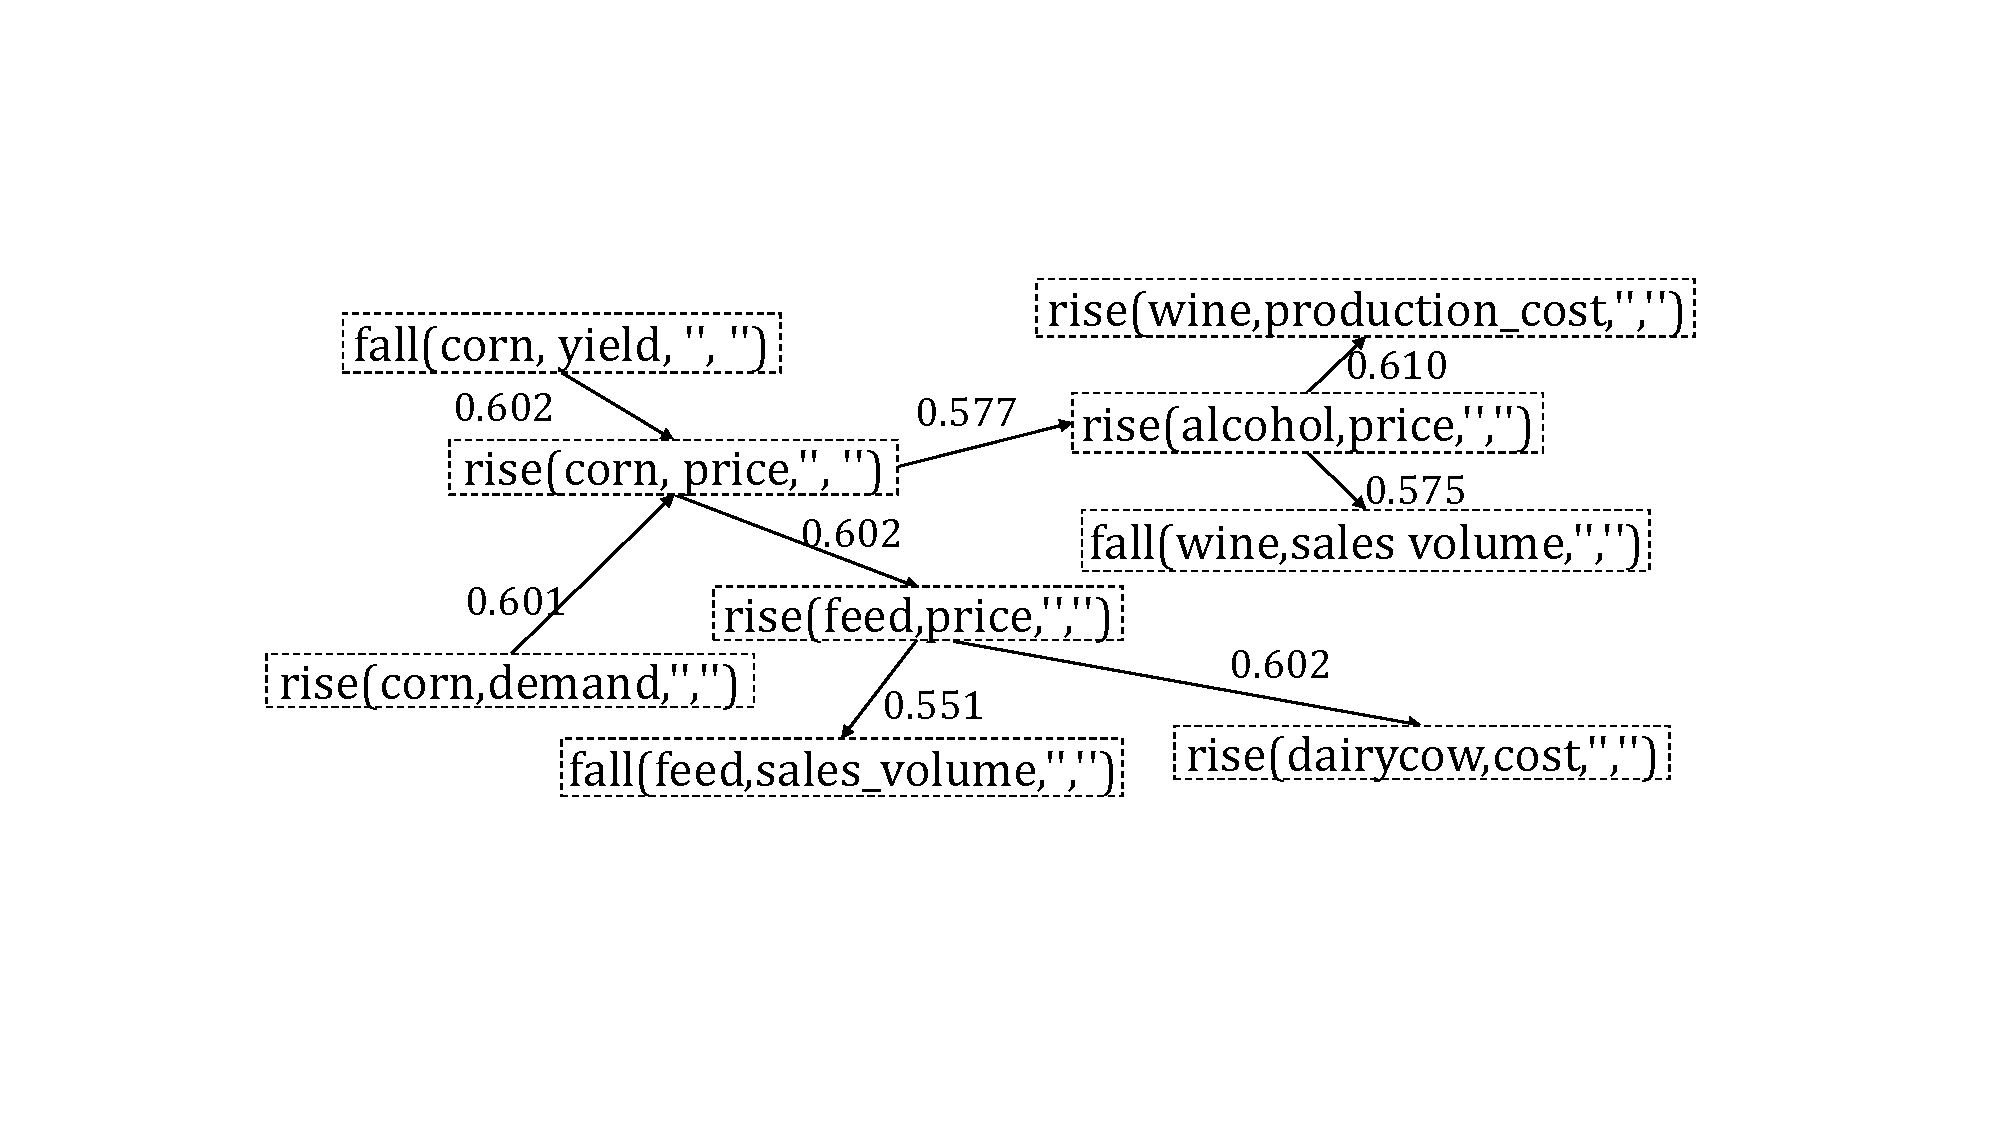
\includegraphics[width=0.9\columnwidth]{figures/instantiation_graph}
	\end{center}
	\caption{Rule Deduction. As space is limited, we only show the English version and omit the rules used in the reasoning process.}
	\label{fig:rule_instantiation_graph}
\end{figure}

\subsection{Downloading and Demo}
\zhpro and \zhcon and learned rules are available at URL.
We built a demo to demonstrate the reasoning process at URL. 

%We also developed an application demo of futures prices change triggering that can monitor news from around the world in real time, find the news that may cause futures prices changes, and alert users. Visit URL.


%
%\subsection{Application: Futures Price Prediction}
%%\paragraph{Reasoning with Uncertainty}
%\begin{figure}[htbp]
%	\begin{center}
%		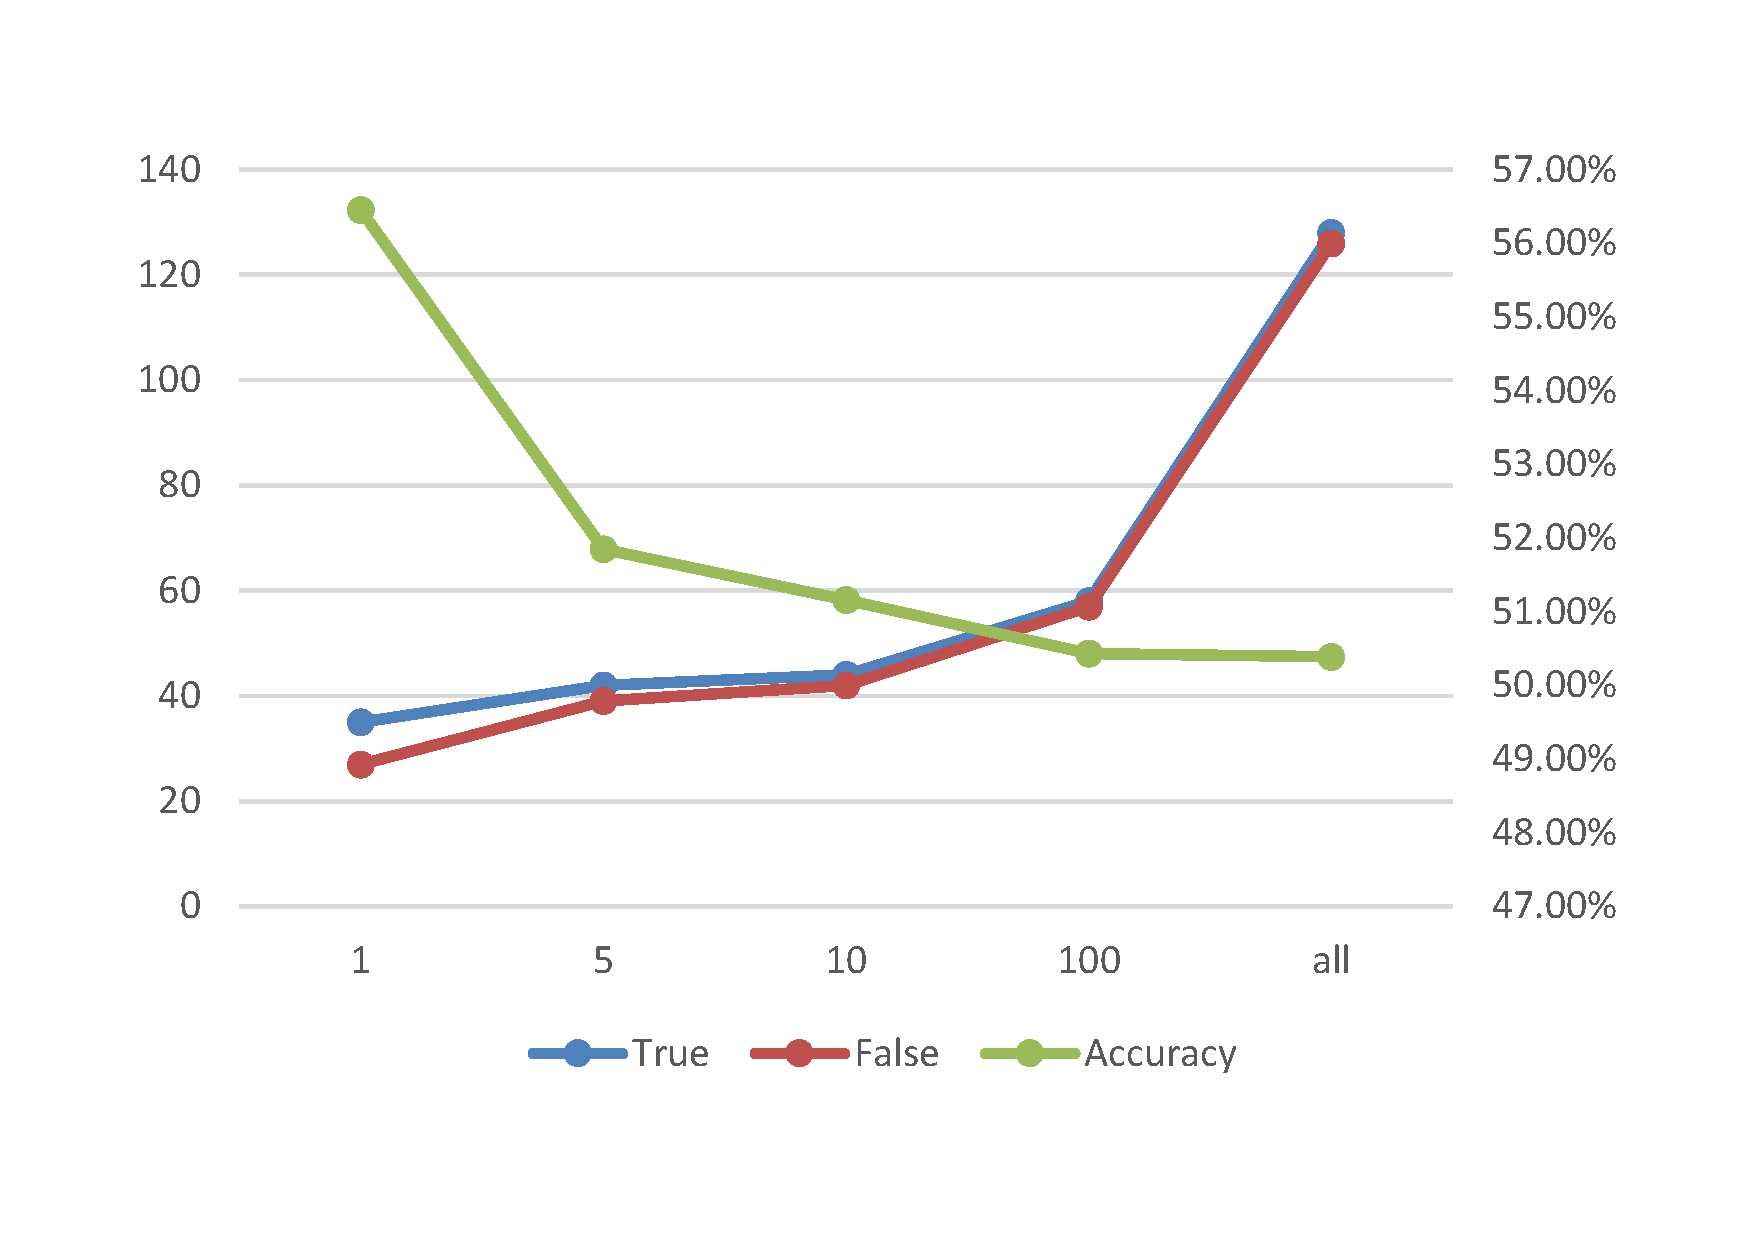
\includegraphics[width=0.9\columnwidth]{figures/rule_futures_prediction}
%	\end{center}
%	\caption{Futures Price Prediction.}
%	\label{fig:futures_price_prediction}
%\end{figure}
%We choose futures price prediction because the futures are common and concrete things existed in ConceptNet and Probase, such as corn, oil, etc.
%%\cite{Ding} is the state-of-the-art stock prediction model(EB\_CNN). We follow similar experimental settings. 
%We follow similar experimental settings in \cite{Ding}.
%From 2018/1/1 to 2018/11/2, we collect all the headlines and the price change of 15 futures as test data, which include \textbf{851} price change events (The price change of more than 1\% relative to the previous day is an event and we only focus on rise or fall events). 
%
%Baseline models: EB\_CNN model \cite{Ding}, the state of the art model in stock price prediction, uses a deep convolutional neural network to model both short-term and long-term influences of events on stock price movements, and the accuracy of futures prediction is \textbf{54.2\%}. Other models in \cite{Ding}, such as EB\_NN, WB\_CNN, and WB\_NN can achieve \textbf{53.0\%}, \textbf{53.2\%}, and \textbf{53.5\%}, respectively. These accuracies of futures prediction are lower than the accuracies of stock prediction shown in the paper.
%It may be because the factors affecting the futures price are far less than the stock price and the futures price is much more stable than the stock price, which makes useful training information about the futures less and further affects the accuracy of the models.
%
%Implementation: For each actual future price change event , we get the news headlines for the previous month before this event. 
%For each news headline, we extract the event, use Prolog to reason based on the rules and external knowledge bases, and get the top K inferred events sorted by the confidence.
%We may have m*K inferred events for this event, m is the number of events occurred in this month. 
%Here, we select the price change events(rise or fall) of the future in this actual future price change event from m*K events and calculate the weighted sum of their confidences(rise event weights 1 and fall event weights -1). If the sum value is positive, we predict this future price as a rise event, otherwise as a fall event. If get no related events changing the future's price, do not make prediction. We compare this prediction with the actual price change to evaluate the reasoning effect. 
%Figure \ref{fig:futures_price_prediction} shows the average prediction result. It shows the more predicted events inferred from the Prolog(by increasing K) we use, the lower the prediction accuracy is(from \textbf{56.5\%} to \textbf{50.4\%}), and the more futures events we can predict(from \textbf{62} to \textbf{254}). 
%
%\textbf{\textit{To sum up}}, our rule-based prediction approach can have a higher prediction accuracy (56.45\%) and better interpretation ability with a low recall rate, which is very practical in life.

%\begin{table}[htbp]
%	\caption{Baselines and Proposed Framework}
%	\begin{center}
%		\begin{tabular}{lll}\hline
%			& Acc & MCC \\\hline
%			WB-NN &  0.535 &     \\
%			WB-CNN&  0.532  &     \\
%			EB-NN &  0.530  &     \\
%			EB-CNN&  0.542   &     \\
%			Rule &     &    \\\hline
%		\end{tabular}
%		\label{tab:baselines_and_rule}
%	\end{center}
%\end{table}